\documentclass[12pt]{report}
\usepackage{graphicx}
\usepackage{float}
\graphicspath{ {images/} }

\begin{document}

\title{Music App Usability Report}
\author{Jeff Fennell}
\date{September 2014}
\maketitle

\section{Intro}

The purpose of this study was to analyze two of the top music applications in existance to determine which has been more optimized for user interaction. 15 different instances of tests were performed on iTunes and Spotify desktop applications. Based on the results, and using efficiency, errors, and satisfaction as metrics for quantifying usability of the two systems, it has been decided that the Spotify platform has been more optimized for user interaction.

The first task the test subjects performed was started on the main music library of the application. Users were asked to create a new playlist with the title "Hello World".  During the second task, users again started on the music library of the application. They were then asked to make use of the automated radio, a feature that is present in both platforms. Users were asked to start the radio and create a station adapted to the artist "Tiesto". Again, the testers were timed to test efficiency of the system. The final task was to havigate to a pre-created playlist on the application, and turn on the playlist to loop indefinitely. For each of the tasks, the amount of time it took each user to complete the task was noted, as well as the number and nature of errors. Users were also asked questions to determine their level of satisfaction with each of the systems.

\section{Efficiency}

Spotify users proved to be more efficient in the first task of creating a playlist. The average time to create a playlist in Spotify was 11.17 seconds, while the average time to perform the same task in iTunes took an average of 16.34 seconds. 4 out of 7 users testing spotify actually completed the task faster than the quickest iTunes time recorded. 3 out of these 4 Spotify testers rated their own familiarity of Spotify as being less than 5 out of 10. This speaks to the learnability of Spotify as well, as users with little domain knowledge were able to quickly complete the task. The iTunes testers' times were slightly higher, with the highest time overall being by an iTunes user who rated their domain knowledge of iTunes as a 9 out of 10. It took this user 26 seconds to create a playlist, a full 7 seconds longer than the slowest time recorded by a Spotify tester. The slowest iTunes tester noted that iTunes frequently updates the user interface, therefore making it difficult to stay familiar with how to use certain features of the software.

\begin{figure}[h]
	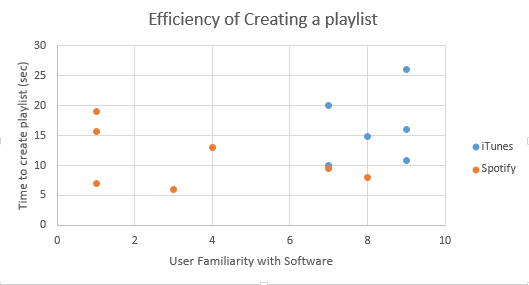
\includegraphics[width=\textwidth]{chart1.png}
	\caption{Average times of completion for each task (lower is better)}
\end{figure}

Test subjects again proved to be much more efficient in performing the second task in Spotfy than in iTunes. The average time to complete the task in Spotify was 23.19 seconds. In iTunes, it generally took test subjects more than 7 seconds longer to complete the task, with the average time being 30.4 seconds. One user additionally commented at this stage that starting a radio station based on a certain artist in Spotify was "easier than iTunes".

The third and final task, starting a playlist and looping it indefinitely, designated Spotify as the more efficient platform. ITunes testers took an average of 38.31 seconds to navigate to and start a playlist looping indefinitely. Spotify users on average took less than half of the time to perform the same task, taking an average of 17.55 seconds.

\section{Errors}

In performing the first task, there were relatively few errors. Again, Spotify yielded better results, with users making only 2 errors during the first task. ITunes testers collectively made 8 errors in the course of the first test. In the second test, iTunes errors made a total of 6 errors, while Spotify users only made 4. On the final task, iTunes testers made 3 errors, while the Spotify users made 4. This puts the total number of errors for the iTunes testers at 17 errors, while the number of errors by Spotify testers was only 10.


\begin{table}[h]
\centering
\begin{tabular}{lllll}
\hline
            & iTunes & Spotify &  &  \\ \hline
First Task  & 8      & 2       &  &  \\
Second Task & 6      & 4       &  &  \\
Third Task  & 3      & 4       &  &  \\ \hline
Total       & 17     & 10      &  & 
\end{tabular}
\end{table}

\section{Satisfaction}

In order to gauge user satisfaction with each of the systems, test subjects were asked after each task how satisfied they were with the ease of completing the task. Additionally, at the end of all three tests, each subject was asked to rate the overall experience in using the platform. It is important to notice the difference between the user-generated overall, and the average between the three tests. The results of the three tests were very close, however, the user-reported overall level of satisfaction proved to be the tiebreaker, with Spotify again coming out as the winner.


\begin{figure}[H]
	\centering
	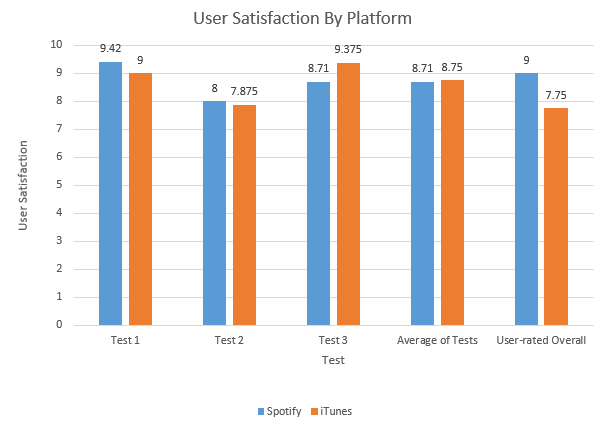
\includegraphics[width=.75\textwidth]{chart2.png}
	\caption{Tester-rated satisfaction with each test, as well as an overall level of satisfaction}
\end{figure}

Figure 2 shows the level of satisfaction users experienced for each task. Users were only slightly more satisfied with Spotify for the first two tests, with an average satisfaction level no more than .4 points higher than the iTunes users. In the third test, iTunes actually scored significantly higher, with a margin of about .6 points separating the two. Regardless of this small victory, users still rated the overall experience of Spotify as more pleasant than that of iTunes, with a margin of 1.25 points. Upon looking at the results, it seems odd that Spotify scored so much higher than iTunes overall. Even though the average satisfaction for the 3 tests was virtually identical. Possible reasons for this difference in rating will be examined in the Heuristics section.


\section{Heuristics}

A very strong possible explanation why Spotify testers had higher levels of satisfaction lies in the average efficiency for each system. As shown in Figure 3, iTune testers took on average, nearly twice as long to perform any one task. While Spotify users took an average of 18.4 seconds per task, iTunes users took a average of 30.47 seconds per task. There is an apparent correlation between the amount of time spent performing tasks, and the overall satisfaction with the system; the longer a user spent performing the same tasks on a system, the lower their satisfaction with the system overall. There are several UI style differences that can account for Spotify being a more efficient system to use.

\begin{figure}[H]
	\centering
	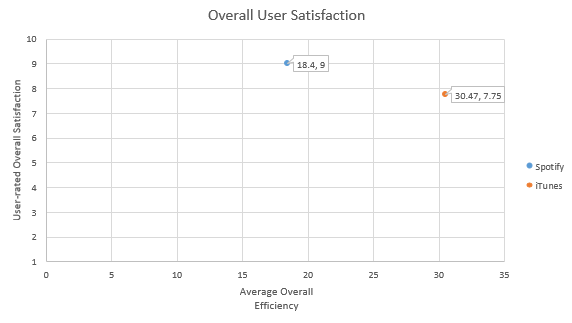
\includegraphics[width=.75\textwidth]{chart3.png}
	\caption{Examining the relationship between average efficiency for all 3 tests, and self-rated overall user satisfaction with system}
\end{figure}

In examining the style of interaction employed by both Spotify and iTunes, some of the reasons that Spotify perform better become apparent. One of the more critical components of the Spotify UI to note is the use of a vertical, scrollable column on the left-hand side of the screen (shown in figure 4). 

\begin{figure}[H]
	\centering
	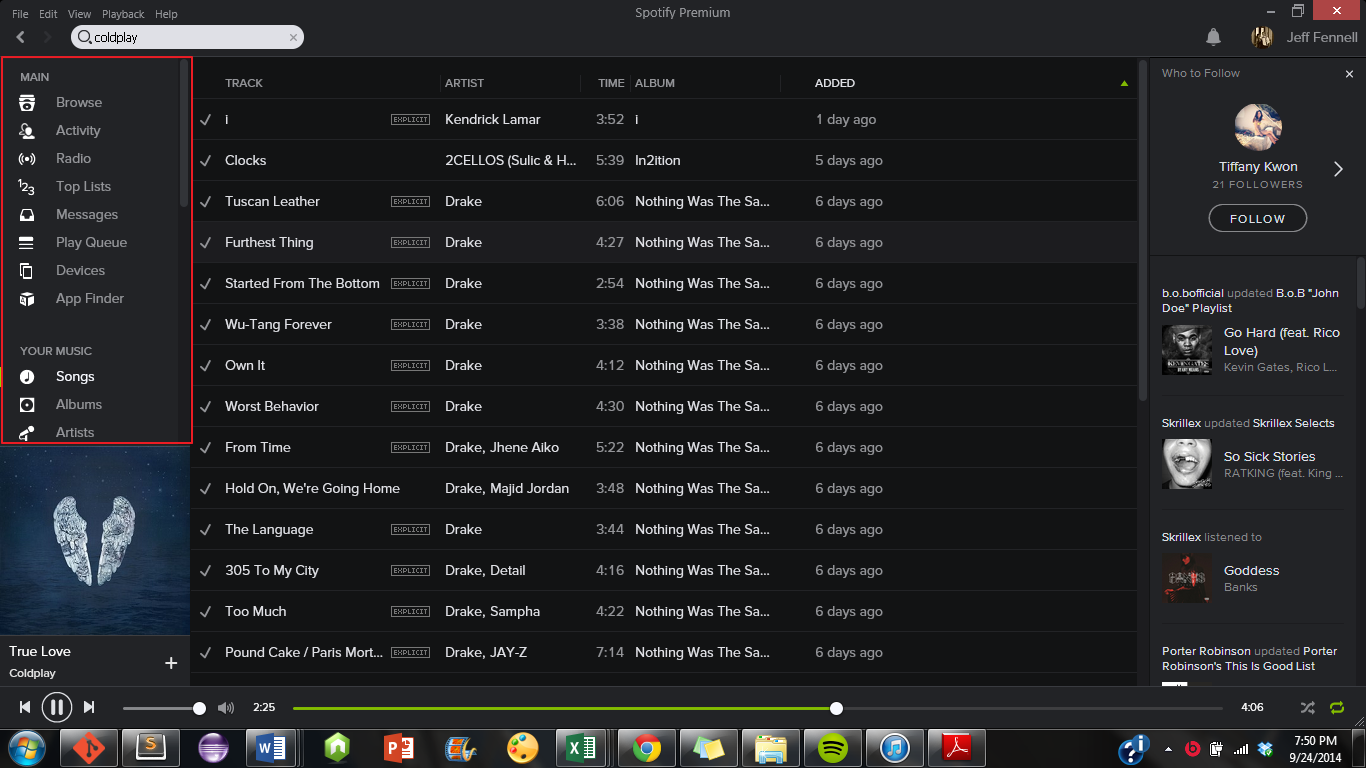
\includegraphics[width=\textwidth]{chart4.png}
	\caption{Spotify employs a navigation column on the left hand side of the screen}
\end{figure}

Here, Spotify holds navigation buttons and commonly used function buttons all in one column. This navigation bar is a permanent fixture in the app, as it remains in place as the user navigates through the system. This navigation bar reduces the number of clicks necessary to navigate through the app. Additionally, the fact that the left-hand side of the navigation bar touches the corner of the window allows the user to navigate to it more quickly. They do not have to worry about overshooting the left hand side of the navigation bar, as the edge of the screen will stop them.

 All three of the tasks we asked users to carry out actually had shortcut buttons in spotify's navigation column. In our first test, many of the users utilized the "create playlist" shortcut in the navigation column to create and name a playlist extremely quickly. This method creates a playlist in one click, immediately allowing the user to type in the name of the new playlist. Even if the user uses the file>create playlist> path, it takes only 2 clicks to create a playlist. Ease of noavigation through this menu bar was also possible in our second task. There is a link in the navigation bar to go straight to the radio function. From there, the user must simply type in the name of the artist to start the radio station. The first hald of the third task was to navigate to a playlist, which the user could do from the navigation column.

iTunes, meanwhile, employs a very thin navigation bar that is not at the top or the side of the window, but rather, dropped slightly towards the center of the screen. This placement and very thin size of the navigatio bar can allow the user to very easily overshoot the navbar when they attempt to click a button. 

\begin{figure}[H]
	\centering
	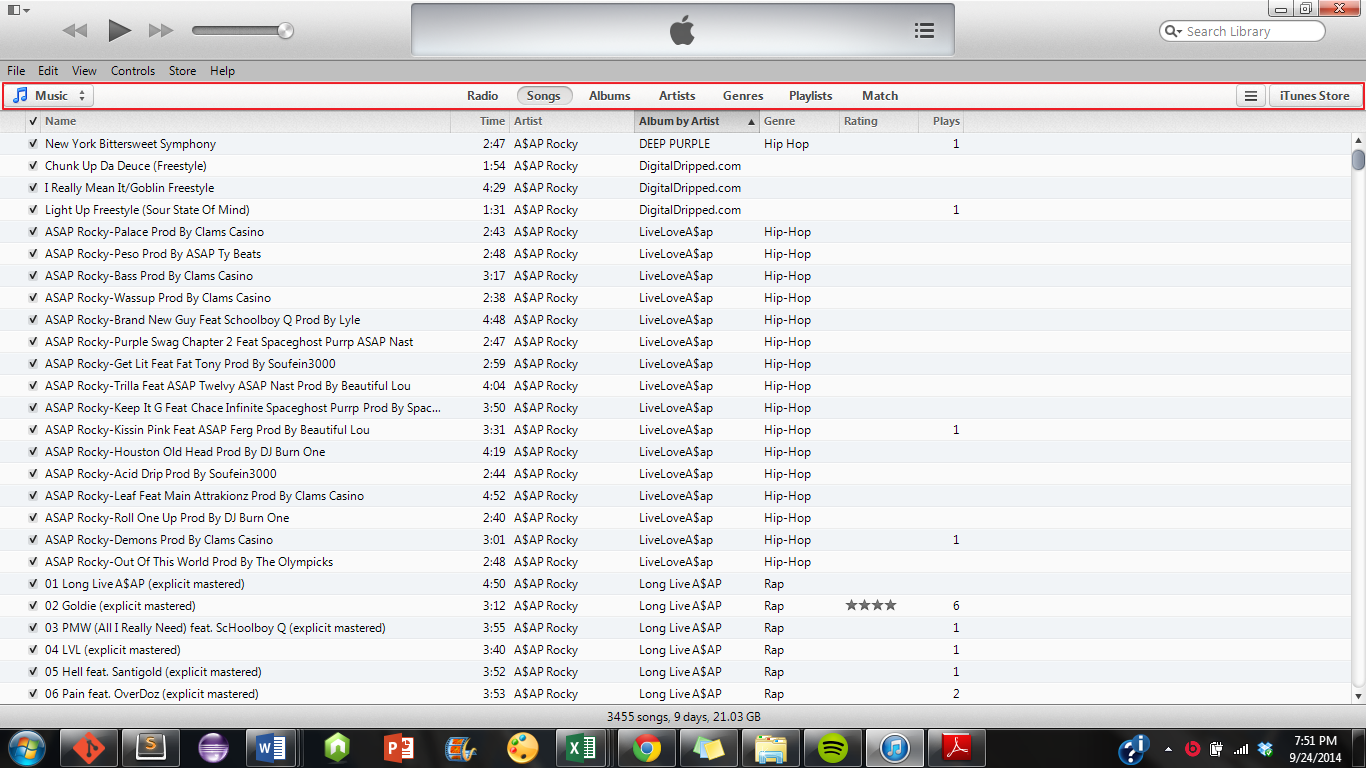
\includegraphics[width=\textwidth]{chart5.png}
	\caption{iTunes employs a horizontal navigation bar with two different drop-down menus, as well as navigation tabs}
\end{figure}

It takes a minimum of 3 mouse clicks to create a playlist in iTunes from the visible buttons in iTunes. From the song library, where the playlist task was started, the user wil likely click the tab labeled "playlists". From this point, however, users must click two more buttons to create a playlist: one button that looks like a plus sign, and then another selecting that the user wants a normal playlist. The second task can again be started in iTunes by using the navigation bar, which again, could be overshot.

Another distinction to be made is the style of buttons in each of the two applications.
-spotify:larger buttons, contain words precisely describing the task they perform
	-buttons that don't have word descriptions:hovering over buttons in spotify pops-up a the button's function
	-many testers accidentally took advantage of this when hesitating to click on a button
-itunes:smaller buttons which could be confused as several possible functions
-mitts law or whatever



\end{document}